%!TEX program=luatex

\newpage
\section{Introduction}
Après avoir finalisé l'étape de conception, nous consacrons ce chapitre à la réalisation. Les différentes problématiques ont étaient profondément analysées, ce qui nous a permit d'entreprendre le développement des modules, ayant comme objectif d'aboutir à un produit final exploitable par les utilisateurs.

Nous allons d'abord présenter l'environnement de travail ainsi que les outils et les logiciels utilisés, nous décrivons également en détails les étapes de réalisation de chaque module, et nous clôturons avec l'évaluation et les résultats de notre système ainsi que l'application mobile réalisée.
\section{Environnement et outils de travail}
    \subsection{Matériels}
    Le matériel utilisé consiste en 2 ordinateurs personnels ainsi qu'un serveur (Cloud) dédié aux traitements gourmands en terme de ressource et en temps d'exécution.
    \begin{enumerate}
        \item{\textbf{Poste de travail 1}}
        \begin{table}[h!]
            \begin{center}
                \begin{tabular}{|C{5cm}|C{8cm}|}
                    \hline
                    \textbf{Système d'exploitation} &  GNU/Linux Ubuntu 16.04 xenial 64bits \\
                    \hline
                    \textbf{RAM} &  4 Go \\
                    \hline
                    \textbf{Processeur} & Intel Core i3-3110M CPU @ 2.4GHz \\
                    \hline
                \end{tabular}
            \end{center}
        \caption{Caractéristiques du poste de travail 1}
        \end{table}

        \item{\textbf{Poste de travail 2}}
        \begin{table}[h!]
            \begin{center}
                \begin{tabular}{|C{5cm}|C{8cm}|}
                    \hline
                    \textbf{Système d'exploitation} &  Windows 8.1 64bits \\
                    \hline
                    \textbf{RAM} &  12 Go \\
                    \hline
                    \textbf{Processeur} & Intel Core i7-5500 CPU @ 2.40 GHZ \\
                    \hline
                \end{tabular}
            \end{center}
        \caption{Caractéristiques du poste de travail 2}
        \end{table}

        \item{\textbf{Serveur (Cloud Virtual Machine)}}
        \begin{table}[h!]
            \begin{center}
                \begin{tabular}{|C{5cm}|C{8cm}|}
                    \hline
                    \textbf{Système d'exploitation} &  GNU/Linux Ubuntu Data Science 64bits \\
                    \hline
                    \textbf{RAM} &  32 Go \\
                    \hline
                    \textbf{Processeur} & Intel Xeon CPU E5-2673 v4 @ 2.295GHz \\
                    \hline
                \end{tabular}
            \end{center}
        \caption{Caractéristiques de la machine virtuelle}
        \end{table}
    \end{enumerate}   

    \subsection{Langages de programmation et logiciels}
    Nous avons utilisé au cours de la réalisation de notre système, plusieurs langages de programmation et logiciels. Ci-après une brève présentation de ces derniers :
        \subsubsection{Langages de programmation}
            \begin{figure}[H]
                    \centering
                    
\includegraphics[height=60pt,width=200pt]{img/chapter4/tools/language.png}
                    \caption{Logos des langages de programmations utilisés}
                    \label{}
            \end{figure}
            \begin{enumerate}
                \item{\textbf{Python : }}
                Python est un langage de programmation de haut niveau. Il supporte la programmation impérative structurée, fonctionnelle et orientée objet. Il est doté d'un typage dynamique fort, d'une gestion automatique de la mémoire. Plusieurs bibliothèques sont fournies afin de faciliter les développements \cite{python}.\\

                \item{\textbf{JavaScript : }}
                Langage de programmation de scripts principalement employé dans les pages web interactives mais aussi pour les serveurs avec l'utilisation (par exemple) de \emph{Node.js}. Il supporte le paradigme objet, impératif et fonctionnel. JavaScript est le langage possédant le plus large écosystème grâce à son gestionnaire de dépendances \emph{npm}, avec environs 500 000 paquets en août 2017 \cite{javascript}.\\

                \item{\textbf{React-Native : }}
                Framework mobile hybride Open source développé par Facebook depuis début 2015. Il continue d'évoluer avec le soutient de nombreux contributeurs. Le but de React Native est de pouvoir réutiliser le maximum de code entre les différentes plate-formes (iOS et Android). Il offre un gain de temps considérable par rapport à du développement spécifique, tout en étant aussi performant \cite{reactnative}.
            \end{enumerate}

        \subsubsection{Librairies et bibliothèques}
            \begin{figure}[h]
                    \centering
                    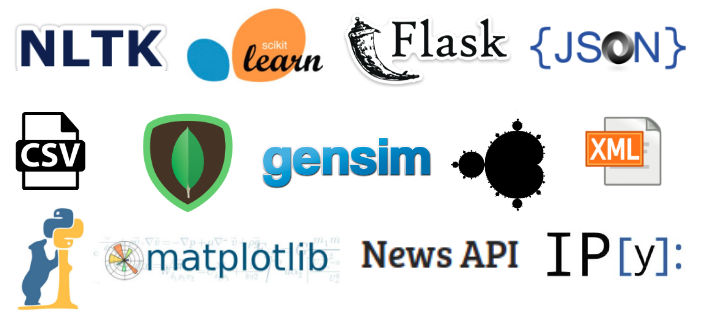
\includegraphics[height=150pt,width=320pt]{img/chapter4/tools/tools.png}
                    \caption{Logos de quelques librairies utilisées}
                    \label{}
            \end{figure}
            \begin{enumerate}
                \item{\textbf{NLTK : }}
                "Natural Language Toolkit" est une librairie python destinée au TALN. Elle fournit une suite de bibliothèques de traitement de texte pour la classification, tokenization, stemming, étiquetage, analyse et raisonnement sémantique, etc. \cite{nltk}.\\

                \item{\textbf{Scikit-Learn : }\label{scikit-learn}}
                Bibliothèque libre et Open source implémenté avec Python, dédiée à l'apprentissage automatique. Elle est conçue pour s'harmoniser avec d'autres bibliothèques Python (ou autres), notamment NumPy, SciPy, etc. \cite{scikit}.\\

                \item{\textbf{Numpy : }}
                "Numerical Python" fournit une interface pour stocker et effectuer des opérations sur les données. D'une certaine manière, les tableaux Numpy sont comme les listes en Python, mais Numpy permet de rendre les opérations beaucoup plus efficaces, surtout sur les tableaux de grande taille qui sont au cœur de l'écosystème de la Data Science \cite{numpy}.\\
                
                \item{\textbf{Gensim : }}
                Librairie Python gratuite conçue pour extraire automatiquement des sujets sémantiques à partir de documents. Les algorithmes de Gensim, tels que l'analyse sémantique latente, permettent de découvrir la structure sémantique des documents en examinant les schémas statistiques de cooccurrence des mots au sein d'un corpus de documents \cite{gensim}.\\

                \item{\textbf{Pandas : }}
                Fournit deux structures de données fondamentales, la "Série" et le "DataFrame". On peut voir ces structures comme une généralisation des tableaux et des matrices de Numpy. La différence entre les structures de Pandas et celles de Numpy c'est la définition explicites par l'utilisateur des indices et des index sur les objets (matrices) .\cite{pandas}\\

                \item{\textbf{Pickle : }}
                Module Python utilisé pour sérialiser et désérialiser les structures d'objets Python. La sérialisation (ou «pickling») fait référence au processus de conversion d'un objet en mémoire en un flux d'octets pouvant être stocké sur disque ou envoyé sur un réseau. Plus tard, ce flux de caractères peut être récupéré et désérialisé (ou «unpickling») en retour vers un objet Python \cite{pickle}.\\

                \item{\textbf{Matplotlib : }}
                "Mathematic Plot library" est une bibliothèque de traçage Python 2D qui produit des figures de qualité de publication dans une variété de formats papier et d'environnements interactifs entre plates-formes. Matplotlib peut être utilisé dans les scripts Python, les Shells Python et IPython, les notebook Jupyter, etc. \cite{matplotlib}.\\

                \item{\textbf{Newspaper : }}
                Librairie python accessible gratuitement qui permet d'extraire le contenu, l'image, les auteurs et la date de publication d'un article de presse en utilisant le protocole HTTP.\\

                \item{\textbf{Newsapi : }}
                Web API qui permet d'obtenir des articles de presse de dernière minute et de recherchez des articles de plus de 30 000 sources et blogs. Elle fournit également la possibilité de sélectionner les sources, les pays, les catégories, etc.\\

                \item{\textbf{FeedParser : }}
                "Universal Feed Parser" est une librairie Python pour le téléchargement et l'analyse des flux syndiqués connu sous l'appellation \emph{flux RSS}. Cette librairie se distingue par sa facilité d'utilisation \cite{feedparser}.\\

                \item{\textbf{TextBlob : }}
                Toolbox Python pour le traitement des données textuelles. Elle fournit une API simple permettant de plonger dans des tâches courantes de TALN, telles que l'étiquetage, l'extraction de syntagmes nominaux, l'analyse des sentiments, la classification, la traduction automatique, etc. \cite{textblob}\\

                \item{\textbf{Farasa : }}
                L'équivalent arabe de "perspicacité", Farasa est une Toolbox de traitement de la langue naturel arabe développé au sein de l'institut \emph{Qatar Computing Research Institute}. Elle est composée de plusieurs modules : segmentation, étiquetage, etc. Farasa surpasse ou égalise les deux fameuses Toolbox pour l'arabe Stanford NLP et MADAMIRA \cite{farasa}.\\

                \item{\textbf{PyRouge : }}
                Interface Python pour le fameux module d'évaluation des résumés automatique ROUGE. Elle facilite l'utilisation de ROUGE avec la conversion des fichiers qui contiennent les résumés en un format interprétable par ROUGE et génère automatiquement les fichiers de configuration ROUGE \cite{pyrouge}.\\

                \item{\textbf{PyMongo}}
                Module de gestion du SGBD MongoDB sous le langage Python, il fournit une variété de commandes très intéressantes qui permettent de faciliter la manipulation d'une base de donnée NoSql \cite{pymongo}.\\
            \end{enumerate}

        \subsubsection{Formats de données}
            \begin{enumerate}
                \item{\textbf{XML : }}
                "eXtensible Markup Language" est un langage informatique de balisage générique. Ces balises permettent de structurer de manière hiérarchisée et organisée les données d'un document.\\

                \item{\textbf{JSON : }}
                "JavaScript Object Notation" est un format adapté aux types de données du langage JavaScript. Au cours des dernières années, JSON est devenu l'un des premiers format d'échange et de stockage de données notamment pour le développement Web \cite{jsonimpl}.\\
                
                \item{\textbf{CSV : }}
                "Comma-separated values" est un format informatique représentant des données tabulaires sous forme de valeurs séparées par des virgules. Le format de fichier CSV est utilisable par les applications de tableur KSpread, OpenOffice Calc, Microsoft Excel, etc. De nombreuses autres applications prennent en charge CSV pour importer ou exporter des données.\cite{csv}
            \end{enumerate}

        \subsubsection{Logiciels et éditeurs de textes}
            \begin{figure}[H]
                    \centering
                    
\includegraphics[height=80pt,width=250pt]{img/chapter4/tools/software.png}
                    \caption{Logos des logiciels utilisés}
                    \label{}
            \end{figure}
            \begin{enumerate}
                \item{\textbf{PyCharm Community Edition : }}
                PyCharm est un éditeur de code pour le développement sous Python, il fournit la complétion de code intelligente, des inspections, la mise en évidence d'erreurs à la volée et des correctifs rapides, ainsi que des corrections de code automatisés et de riches fonctionnalités de navigation.\cite{pycharm} Le version \emph{Community Edition} que nous avons utilisé est gratuite et en libre accès.\\

                \item{\textbf{WebStorm : }}
                WebStorm est un éditeur de code pour le développement sous Javascript, il apporte une aide énorme au développeurs Web et mobile. Il supporte tout les langages compilés au JavaScript, Node.js, HTML et CSS \cite{webstorm}. Nous avons pu obtenir une licence étudiant d'une année.\\

                \item{\textbf{Sublime Text : }}
                Éditeur de texte générique codé en C++ et Python, disponible sur Linux, Mac et Windows. Depuis la version 2.0, sortie le 26 juin 2012, l'éditeur prend en charge 44 langages de programmation majeurs, tandis que des plugins sont souvent disponibles pour les langages plus rares \cite{sublime}. Nous avons utilisé la version d’essai qui est en libre accès sur internet.\\

                \item{\textbf{Git : }}
                Système de gestion de versions décentralisé. C'est un logiciel libre créé par \emph{Linus Torvalds}, auteur du noyau Linux, et distribué selon les termes de la licence publique générale (GPL). En 2016, il s’agit du logiciel de gestion de versions le plus populaire qui est utilisé par plus de douze millions de personnes \cite{git}.
            \end{enumerate}


\section{Catégorisation}
    Le premier module sur lequel nous avons travailler, c'est la catégorisation d'articles de presse. Nous avons expérimenter plusieurs techniques proposées dans la littérature. Nous présentons ci-après chaque approche, ses résultats, ses points forts et ses faiblesses.
    \subsection{Approches utilisées\label{approches}}
        Toutes les approches utilisées sont basées sur l'apprentissage automatique, supervisé et non supervisé. 
        \subsubsection{Basées sur l'Apprentissage Non Supervisé}
            \begin{itemize}
                \item{LDA (Latent Dirichlet Allocation) : }
                \item{K-means : }
            \end{itemize}

        \subsubsection{Basées sur l'Apprentissage Supervisé}
            \begin{itemize}
                \item{Naïve de Bayes : }
                c'est une méthode connue de l'Apprentissage automatique supervisé. Un de ses avantages en plus d'être un modèle simple, c'est qu'ils renvoient non seulement la prédiction mais aussi le degré de certitude, ce qui peut être très utile dans certaines applications. Mais en ayant un problème à classes multiples, cette approche nous a donnés des résultats très modeste en un temps d'exécution assez importants, ce qui nous a poussé à abandonner son utilisation.\\

                \item{Arbres de décision : }
                peuvent être assistés par un expert. Ces principaux avantages sont : robuste face aux données aberrantes, pas très sensible aux données manquantes, possibilité d’intervenir dans la construction de l’arbre, etc. Son principale inconvénient reste la dépendance très forte entre la taille de la base d’apprentissage et les performances.\\

                \item{Réseaux de neurones : }
                \item{SVM (Support Vector Machines) : }
                \item{Descente de Gradient Stochastique : }
            \end{itemize}
                
    \subsection{Corpus et dataset}
        Comme tout problème de classification, la catégorisation d'articles de presse nécessite de très grandes masses de données. C'est pour cela que nous avons consacrer une bonne période du projet à la récolte des corpus et la préparation des datasets.     
        \subsubsection{Quelques chiffres et statistique}
            \begin{itemize}
                \item{\textbf{Anglais : }}
                 Le dataset baptisé "News" a été récolté par le Laboratoire Informatique de \emph{l'Université de Pise} \cite{pise}, il regroupes des articles de 3 sources différentes : \emph{The New York Times}, \emph{Reuters} et \emph{USA Today}. le Tableau \ref{news-categ} présente en détails le nombre d'articles de chaque catégorie.
                \begin{table}[H]
                    \begin{center}
                        \begin{tabular}{|C{5cm}|C{5cm}|}
                            \hline
                            \textbf{Catégorie} &  \textbf{Nombre d'articles} \\
                            \hline
                            Business & 5366 \\
                            \hline
                            Entertainment & 3286 \\
                            \hline
                            Health & 1851 \\
                            \hline
                            Science \& Technology & 2872 \\
                            \hline
                            Sport & 8189 \\
                            \hline
                            US & 4783 \\
                            \hline
                            World & 6255 \\
                            \hline
                            \textbf{Totale} &  \textbf{32602} \\
                            \hline
                        \end{tabular}
                    \end{center}
                    \caption{Nombres d'articles de chaque catégorie du corpus "News"}
                    \label{news-categ}
                \end{table}
                \item{\textbf{Arabe : }}
                Le corpus TALAA\footnote{Traitement Automatique du Langage et Apprentissage Automatique, l'équipe de recherche du Laboratoire de Recherche en Intelligence Artificielle du département informatique de l'USTHB} pour la catégorisation d'articles de presse est une grande collection d'articles publiés à partir de 2010 jusqu'à 2014 dans différentes revue de presse sur internet. Il contient plus de 14 millions de mots de 582000 types différents. Le corpus contient 8 catégories, mais nous avons choisi de travailler sur 6 catégories plus générales comme on peut le constater dans le tableau suivant \ref{talaa-categ} \cite{talaa}. 
                \begin{table}[H]
                    \begin{center}
                        \begin{tabular}{|c|c|}
                            \hline
                            \textbf{Catégorie} &  \textbf{Nombre d'articles} \\
                            \hline
                            \begin{arab}الجزائر\end{arab} & 6603 \\
                            \hline
                            \begin{arab}الثقافة\end{arab} & 3311 \\
                            \hline
                            \begin{arab}الدين\end{arab} & 2568 \\
                            \hline
                            \begin{arab}المجتمع\end{arab} & 7714 \\
                            \hline
                            \begin{arab}الرياضة\end{arab} & 8104 \\
                            \hline
                            \begin{arab}العالم\end{arab} & 4380 \\
                            \hline
                            \textbf{Totale} & \textbf{32680} \\
                            \hline
                        \end{tabular}
                    \end{center}
                    \caption{Nombres d'articles des 6 catégories choisies du corpus "TALAA"}
                    \label{talaa-categ}
                \end{table}
            \end{itemize}
        \subsubsection{Pré-traitement et structure des datasets}
            Les deux corpus utilisés pour les deux langues étaient sous le format brute, ce qui nécessitaient une restructuration et un pré-traitement afin de permettre leur exploitation.  

            Plusieurs opérations de pré-traitements ont été effectuées. Ci-après les étapes suivies :
            \begin{enumerate}
                \item{\textbf{Segmentation (Tokenization) et suppression des mots vides :} }permet d'extraire toutes les entités lexicales d'un article donné. Pour l'Anglais nous avons utiliser le Tokenizer natif de NLTK, et FARASA Toolbox pour la langue Arabe. La segmentation est suivie de la suppression des tokens non utiles tel que la ponctuation, les pronoms, les déterminants, etc.\\  
                
                \item{\textbf{Racinisation (Stemming) :} }les mots d'un document sont représentés par leurs racines plutôt que par les mots d'origine. Plusieurs variantes d'un terme peuvent ainsi être groupées dans une seule forme représentative, ce qui réduit le nombre des termes distincts nécessaires pour représenter un document. Le Snowball Stemmer a été utilisé pour l'Anglais, quant à l'Arabe c'est toujours la Toolbox FARASA.\\

                \item{\textbf{N-grammes :} }les N-grammes permettent de construire une sous-séquence de n mots consécutives. Ils permettent de contextualiser l'ordre d'apparition d'un ensemble de mots. L'algorithme natif de NLTK a été utilisé pour les deux langues (Anglais et Arabe).\\ 
                
                \item{\textbf{Extraction des caractéristiques :} }avec l'utilisation de TF-IDF, le sac de mots représentant un article sera convertit en valeurs numériques décrivant la fréquence d'occurrence de chaque mot par rapport à l'ensemble des articles du corpus et à l'article lui même.\\
            \end{enumerate}

            À la fin de la phase de pré-traitement, nous avons définie une structure pour faciliter l'exploration des datasets. Ci-dessous la structure choisie :
                \begin{itemize}
                    \item{\textbf{id} :}un identifiant unique de l'article,
                    \item{\textbf{contenu} :}les différents paragraphes de l'article,
                    \item{\textbf{catégorie} :}la catégorie de l'article extraite depuis la source.
                \end{itemize}
    \subsection{Modèles finaux}
        Après expérimentation des techniques citées dans \ref{approches}, voici les modèles finaux de la catégorisation d'articles de presse implémentés en Python en utilisant la librairie Scikit-learn \ref{scikit-learn} :
        \begin{itemize}
            \item{\textbf{Anglais :} }le modèle le plus performant est obtenu en utilisant l'algorithme SVM avec 80\% de données pour l'apprentissage et le 20\% restant pour les tests sur un total de 32602 articles de 7 catégories différentes.\\

            \item{\textbf{Arabe :} }l'algorithme de la Descente de Gradient Stochastique nous a donné les meilleurs résultats en utilisant 32680 articles, avec 75\% de données pour l'apprentissage et le reste pour les tests. 
        \end{itemize}
    \subsection{Résultats et évaluation}
        \subsubsection{Métriques d'évaluations}
            \begin{itemize}
                \item{\textbf{Accuracy :} }c'est une mesure qui évalue l'efficacité globale de l'algorithme par rapport au données de test.
                    \[ Accuracy = \frac{tp+tn} {tp+fp+tn+fn} \]
                \item{\textbf{Précision :} }elle évalue le pouvoir prédictif du modèle en mesurant la capacité du modèle à prédire que des classes correctes.
                    \[ Precision = \frac{tp} {tp+fp} \]
                \item{\textbf{Rappel :} }la capacité d’un modèle à prédire toutes les classes correctes de l'ensemble de test.
                    \[ Rappel = \frac{tp} {tp+fn} \]
                \item{\textbf{F-mesure :} }une mesure composite qui profite aux algorithmes avec une sensibilité plus élevée et des algorithmes de défis avec spécificité plus élevée.!!!
                    \[ F-mesure = \frac{2 * (Precision * Rappel)} {(Precision + Rappel)} \]
            \end{itemize}
            Avec :
            \begin{itemize}
                \item{\textbf{TP }True Positive (vrais positifs) :} nombre d'individus bien prédits dans la classe à juste titre.
                \item{\textbf{FP }False Positive (faux positifs) :} nombre d'individus prédits d'une classe alors qu'ils ne devraient pas en faire parti.
                \item{\textbf{FN }False Negative (faux négatifs) :} nombre d'individus prédits comme étant de la classe alors qu'il ne le sont pas en vrai.
                \item{\textbf{TN }True Negative (vrais négatifs) :} nombre d'individus prédits comme n'étant pas dans la classe à juste titre.
            \end{itemize}

        \subsubsection{Résultats}
        \begin{itemize}
            \item{\textbf{Anglais :}}
            \begin{itemize}
                \item{Accuracy : 0.987}
                \item{Précision : 0.988}
                \item{Rappel : 0.982}
                \item{F-mesure : 0.985}
            \end{itemize}
            \begin{table}[H]
                    \begin{center}
                        \begin{tabular}{|c|C{2cm}|C{2cm}|C{2cm}|C{2cm}|}
                            \hline
                            \textbf{Catégorie} &  \textbf{Précision} &  \textbf{Rappel} &  \textbf{F-mesure} &  \textbf{Support} \\
                            \hline
                            Business & 0.98 & 0.96 & 0.97 & 1046 \\
                            \hline
                            Entertainment & 0.99 & 0.99 & 0.99 & 651 \\
                            \hline
                            Health & 0.97 & 1.00 & 0.99 & 388 \\
                            \hline
                            Science \& Technology & 0.94 & 1.00 & 0.97 & 546 \\
                            \hline
                            Sport & 1.00 & 1.00 & 1.00 & 1635 \\
                            \hline
                            US & 0.99 & 0.98 & 0.99 & 993 \\
                            \hline
                            World & 1.00 & 0.99 & 0.99 & 1262 \\
                            \hline                            
                            \textbf{Moyenne/Totale} & \textbf{0.99} & \textbf{0.98} & \textbf{0.99} & \textbf{6521} \\
                            \hline
                        \end{tabular}
                    \end{center}
                    \caption{Résultat global et pour chaque catégorie de la catégorisation pour l'Anglais}
            \end{table}
            \item{\textbf{Arabe :}}
            \begin{itemize}
                \item{Accuracy : 0.936}
                \item{Précision : 0.94}
                \item{Rappel : 0.94}
                \item{F-mesure : 0.94}
            \end{itemize}
            \begin{table}[H]
                    \begin{center}
                        \begin{tabular}{|c|C{2cm}|C{2cm}|C{2cm}|C{2cm}|}
                            \hline
                            \textbf{Catégorie} &  \textbf{Précision} &  \textbf{Rappel} &  \textbf{F-mesure} &  \textbf{Support} \\
                            \hline
                            \begin{arab}الجزائر\end{arab} & 0.93 & 0.88 & 0.91 & 664 \\
                            \hline
                            \begin{arab}الثقافة\end{arab} & 0.91 & 0.86 & 0.88 & 509 \\
                            \hline
                            \begin{arab}الدين\end{arab} & 0.94 & 0.92 & 0.93 & 860 \\
                            \hline
                            \begin{arab}المجتمع\end{arab} & 0.91 & 0.94 & 0.92 & 1541 \\
                            \hline
                            \begin{arab}الرياضة\end{arab} & 0.99 & 0.99 & 0.99 & 1620 \\
                            \hline
                            \begin{arab}العالم\end{arab} & 0.92 & 0.94 & 0.93 & 1316 \\
                            \hline                            
                            \textbf{Moyenne/Totale} & \textbf{0.94} & \textbf{0.94} & \textbf{0.94} & \textbf{6510} \\
                            \hline
                        \end{tabular}
                    \end{center}
                    \caption{Résultat global et pour chaque catégorie de la catégorisation pour l'Arabe}
                \end{table}
        \end{itemize}

        \subsubsection{Évaluations}
        \begin{itemize}
            \item{\textbf{Anglais :} }
            \begin{itemize}
                \item{Matrice de confusions : }
                \begin{table}[H]
                    \begin{center}
                        \begin{tabular}{|c|c|c|c|c|c|c|c|}
                            \hline
                            \textbf{VIDE} & \textbf{Sport} &  \textbf{World} &  \textbf{News} &  \textbf{Business} &  \textbf{Health} & \textbf{Entert.\footnote{Entertainment}} &  \textbf{Sci-Tech} \\
                            \hline
                            \textbf{Sport} & 1635 & 0 & 0 & 0 & 0 & 0 & 0 \\
                            \hline
                            \textbf{World}  & 0 & 1249 & 0 & 9 & 2 & 1 & 1 \\
                            \hline
                            \textbf{News}  & 0 & 0 & 974 & 11 & 3 & 3 & 2 \\
                            \hline
                            \textbf{Business}  & 0 & 5 & 4 & 1003 & 3 & 0 & 31 \\
                            \hline
                            \textbf{Health}  & 0 & 0 & 0 & 0 & 388 & 0 & 0 \\
                            \hline
                            \textbf{Entert.}  & 0 & 0 & 0 & 1 & 3 & 646 & 1 \\
                            \hline
                            \textbf{Sci-Tech}  & 0 & 0 & 1 & 0 & 0 & 1 & 544 \\
                            \hline
                        \end{tabular}
                    \end{center}
                    \caption{Matrice de confusion du modèle de la catégorisation d'articles Anglais}
                \end{table}
                % \item{Courbe ROC : }
                % \begin{figure}[H]
                %     \centering
                %     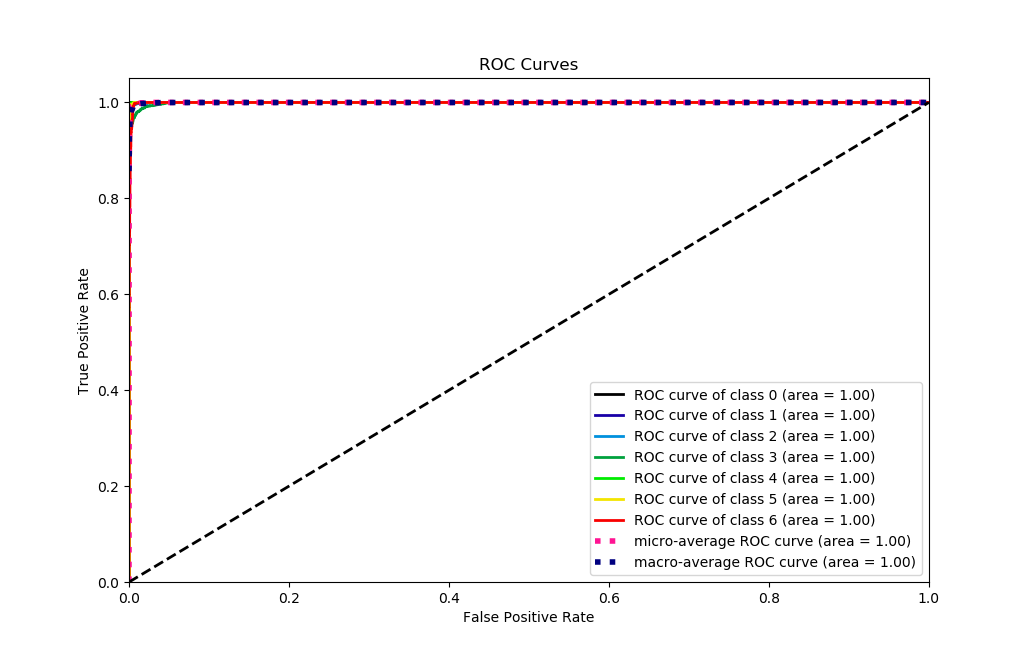
\includegraphics[height=320pt,width=330pt]{img/chapter4/rocEN.png}
                %     \caption{}
                %     \label{}
                % \end{figure}
            \end{itemize}
            \item{\textbf{Arabe :} }
                \item{Matrice de confusions : }
                \begin{table}[H]
                    \begin{center}
                        \begin{tabular}{|c|c|c|c|c|c|c|}
                            \cline{2-7}
                            \hline
                            \multicolumn{1}{c|}{} & \multicolumn{6}{|c|}{Predicted} \\
                            \hline
                            \multicolumn{1}{c|}{} & \textbf{\begin{arab}العالم\end{arab}} &  \textbf{\begin{arab}الرياضة\end{arab}} &  \textbf{\begin{arab}الجزائر\end{arab}} &  \textbf{\begin{arab}المجتمع\end{arab}} &  \textbf{\begin{arab}الدين\end{arab}} &  \textbf{\begin{arab}الثقافة\end{arab}} \\
                            \hline
                            \textbf{\begin{arab}العالم\end{arab}} & 1232  &  1  & 11 &  51  & 18  &  3 \\
                            \hline
                            \textbf{\begin{arab}الرياضة\end{arab}}  & 1 & 1609  &  1  &  6  &  3 &   0 \\
                            \hline
                            \textbf{\begin{arab}الجزائر\end{arab}}  & 28  &  2 & 587 &  21  &  9  & 17 \\
                            \hline
                            \textbf{\begin{arab}المجتمع\end{arab}}  & 43  & 11 &  17& 1447 &  12 &  11 \\
                            \hline
                            \textbf{\begin{arab}الدين\end{arab}}  & 36  &  0  &  6 &  18 & 788 &  12 \\
                            \hline
                            \textbf{\begin{arab}الثقافة\end{arab}}  & 3  &  0 &   8 & 53  &  9 & 436 \\
                            \hline
                        \end{tabular}
                    \end{center}
                    \caption{Matrice de confusion du modèle de la catégorisation d'articles Arabe}
                \end{table}

                % \item{Courbe ROC : }
                % \begin{figure}[H]
                %     \centering
                %     \includegraphics[height=320pt,width=330pt]{img/chapter4/ux/1.png}
                %     \caption{}
                %     \label{}
                % \end{figure}
        \end{itemize}

\section{Résumé automatique}
    Le deuxième module que nous avons développé est le module de résumé automatique, en eefet comme pour le module de recommandation, nous avons choisi \emph{Python} pour le développer.\\
    \subsection{Approches utilisées}
        \subsubsection{Résumé extractif par Apprentissage Supervisé}
            \begin{itemize}
                \item{\textbf{Corpus et datasets}}
                \item{\textbf{Pré-traitement et structure des datasets}}
                \item{\textbf{Faiblesse et critique}}
            \end{itemize}
        \subsubsection{Résumé extractif par Machine de Boltzman}
            L'approche proposée dans \cite{boltzman} utilise un modèle d'apprentissage profond.   
            \begin{itemize}
                \item{\textbf{Pré-traitement et structure des datasets}}
                \item{\textbf{Faiblesse et critique}}
            \end{itemize}
        \subsubsection{Résumé extractif par Plongement de mots\ref{plongement}}
                % \item{\textbf{Pré-traitement des données}}
    \subsection{Résultats et évaluation}
        \subsubsection{Métrique d'évaluation}
        \title{Anglais}
        \title{Arabe}

\section{Recommandation}
    \subsection{Approches utilisées}    
    \subsection{Résultats et évaluation}
        \subsubsection{Métrique d'évaluation}